\documentclass[11pt,a4paper]{article}

% Encoding and fonts
\usepackage[utf8]{inputenc}
\usepackage[T1]{fontenc}
\usepackage{lmodern}
\usepackage{microtype}

% Page layout
\usepackage[margin=2.5cm]{geometry}
\usepackage{setspace}
\setstretch{1.08}

% Math
\usepackage{amsmath,amssymb}

% Graphics and tables
\usepackage{graphicx}
\usepackage{booktabs}
\usepackage{multirow}
\usepackage{array}
\usepackage{caption}
\usepackage{subcaption}
\usepackage{xcolor}
\usepackage{enumitem}

% Code listings
\usepackage{listings}
\lstset{
  basicstyle=\ttfamily\small,
  breaklines=true,
  frame=single,
  backgroundcolor=\color{gray!10},
  numbers=none,
  xleftmargin=0.5em,
  xrightmargin=0.5em,
}

% Diagrams
\usepackage{tikz}
\usetikzlibrary{shapes.geometric, arrows.meta, positioning, fit, backgrounds, calc}

% Hyperlinks
\usepackage{hyperref}
\usepackage{cleveref}
\hypersetup{
  colorlinks=true,
  linkcolor=blue,
  citecolor=blue,
  urlcolor=blue,
}

% Convenience commands
\newcommand{\tool}[1]{\texttt{#1}}
\newcommand{\modelname}{\tool{yolo26n-seg}}

\title{\textbf{YOLO26-Based Road Instance Segmentation:\\A Reproducible Lightweight Pipeline for Autonomous Driving Perception}}
\author{Author Name$^{1}$ \\ $^{1}$Department of Computer Science, Institution Name \\ \texttt{author@example.edu}}
\date{July 2026}

\begin{document}

\maketitle

\begin{abstract}
Road instance segmentation is a core perception task in autonomous driving: it predicts the exact pixel-level boundary of the drivable area from a forward-facing camera. We present a reproducible, end-to-end pipeline for single-class road instance segmentation in driving-scene images. Built on Ultralytics YOLO v8.4.112, we fine-tune a lightweight \modelname{} model initialized with COCO-seg pre-trained weights. Our custom dataset contains 100 polygon-annotated road images extracted from on-board videos, split into 80 training, 10 validation, and 10 test images. We adopt a frozen-backbone transfer-learning strategy (the first 10 layers are frozen), high-resolution training at 960\,px, and a custom dataset checker that guarantees annotation integrity before training. On the validation set, the best model achieves box mAP@0.5 = 0.995, mask mAP@0.5 = 0.995, box mAP@0.5:0.95 = 0.950, and mask mAP@0.5:0.95 = 0.879. Ablation studies show that freezing the backbone consistently improves generalization on our small dataset compared with full fine-tuning. The entire pipeline, including environment bootstrapping, data preparation, training, validation, inference, and ONNX export, is scripted and timestamped for full reproducibility.
\end{abstract}

\section{Introduction}\label{sec:intro}

Autonomous driving systems must perceive the road surface accurately and in real time. While object detection answers the question ``what and where,'' instance segmentation additionally provides the precise contour of each object, which is essential for motion planning and free-space estimation. Among driving-scene objects, the drivable road region is arguably the most important single class: knowing its exact boundary allows a vehicle to stay in lane, avoid curbs, and plan trajectories within a safe corridor.

Classical road segmentation relied on hand-crafted color and texture features, often combined with vanishing-point or lane-line heuristics. These methods struggle with shadows, wet surfaces, varying pavement colors, and unstructured roads. Deep-learning approaches, especially fully convolutional networks (FCNs) \cite{Long2015FCN} and encoder--decoder architectures such as U-Net \cite{Ronneberger2015UNet}, have substantially improved robustness by learning features directly from data. More recently, one-stage detectors in the YOLO family \cite{Redmon2018YOLOv3,Bochkovskiy2020YOLOv4,Jocher2023Ultralytics} have been extended with parallel mask branches to perform instance segmentation at high frame rates, making them attractive for edge deployment in vehicles.

Despite these advances, building a reproducible road-segmentation pipeline remains nontrivial. Practitioners must manage heterogeneous software dependencies, convert raw video into labeled datasets, validate annotations, tune hyperparameters for small datasets, and export models to deployment formats. This project addresses these engineering challenges by delivering:
\begin{itemize}[leftmargin=2em]
    \item a fully scripted pipeline from environment setup to ONNX export;
    \item a custom dataset checker that verifies image--label pairing, normalized polygon coordinates, and non-zero polygon area;
    \item a frozen-backbone transfer-learning strategy tailored to a 100-image road dataset;
    \item quantitative ablation studies on backbone freezing and inference resolution, plus qualitative validation visualizations.
\end{itemize}

\section{Background}\label{sec:background}

\subsection{Road segmentation in autonomous driving}

Road segmentation can be formulated either as semantic segmentation, where every pixel is classified as road or non-road, or as instance segmentation, where individual road instances are detected and masked. For a single-class drivable-region task, the two formulations coincide except that an instance-segmentation model also emits a bounding box and confidence score, which are useful for downstream fusion and uncertainty estimation. Public driving datasets such as BDD100K \cite{Yu2020BDD100K} and Cityscapes provide diverse road labels, but domain-specific onboard footage often has different camera intrinsics, mounting heights, and road types, making custom datasets necessary.

\subsection{YOLO-family instance segmentation}

You Only Look Once (YOLO) detectors frame object detection as a single regression problem over a grid of anchor or anchor-free cells. Modern YOLO variants, including YOLOv4 \cite{Bochkovskiy2020YOLOv4} and Ultralytics YOLOv8 \cite{Jocher2023Ultralytics}, add a semantic mask branch that produces coarse prototype masks combined with per-instance mask coefficients. The resulting architecture jointly optimizes box, class, and mask losses, yielding both detection and instance-segmentation outputs in one forward pass. Mask R-CNN \cite{He2017MaskRCNN} remains a strong two-stage alternative, but its region-proposal stage is slower and less suitable for real-time automotive perception.

\subsection{Transfer learning and backbone freezing}

Training deep networks from scratch requires large annotated datasets. Transfer learning mitigates data scarcity by initializing a model with weights learned on a large source dataset such as MS COCO \cite{Lin2014COCO} and then fine-tuning on a target domain. In backbone--neck--head architectures, low-level backbone features (edges, textures) transfer well across visual domains, whereas high-level neck and head features are task- or domain-specific. Freezing the backbone and only updating the neck and head reduces the number of trainable parameters, lowers overfitting risk, and shortens training time when the target dataset is small \cite{Jocher2023Ultralytics}.

\subsection{Evaluation metrics}\label{sec:metrics}

We adopt the COCO-style mean average precision (mAP). For a predicted mask or box $A$ and a ground-truth mask or box $B$, the Intersection over Union (IoU) is
\begin{equation}\label{eq:iou}
    \text{IoU}(A,B) = \frac{|A \cap B|}{|A \cup B|}.
\end{equation}
A prediction is a true positive if IoU exceeds a given threshold and the class matches. \text{mAP@0.5} averages precision across recall levels at IoU$=0.5$, while \text{mAP@0.5:0.95} averages AP over ten IoU thresholds from 0.5 to 0.95 in steps of 0.05. We report both box and mask variants.

\section{Method}\label{sec:method}

\subsection{Pipeline overview}

Our project is organized as a linear, reproducible pipeline:
\begin{center}
\small
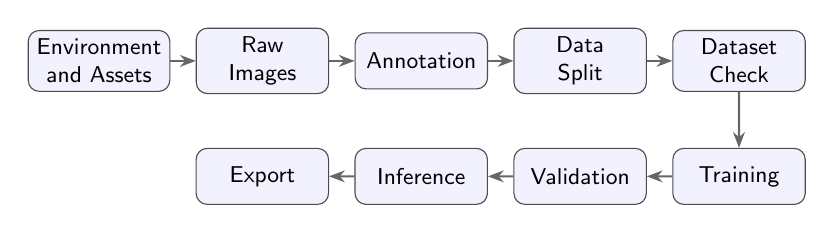
\begin{tikzpicture}[
    node distance=1.0em,
    box/.style={rectangle, rounded corners, draw=black!70, fill=blue!5, minimum width=5.2em, minimum height=2.2em, align=center, font=\sffamily\small},
    arrow/.style={-{Stealth[length=2mm]}, thick, black!60},
    scale=0.92, transform shape
]
\node[box] (env) {Environment\\and Assets};
\node[box, right=of env] (raw) {Raw\\Images};
\node[box, right=of raw] (ann) {Annotation};
\node[box, right=of ann] (split) {Data\\Split};
\node[box, right=of split] (check) {Dataset\\Check};
\node[box, below=2.2em of check] (train) {Training};
\node[box, left=of train] (val) {Validation};
\node[box, left=of val] (pred) {Inference};
\node[box, left=of pred] (exp) {Export};

\draw[arrow] (env) -- (raw);
\draw[arrow] (raw) -- (ann);
\draw[arrow] (ann) -- (split);
\draw[arrow] (split) -- (check);
\draw[arrow] (check) -- (train);
\draw[arrow] (train) -- (val);
\draw[arrow] (val) -- (pred);
\draw[arrow] (pred) -- (exp);
\end{tikzpicture}
\end{center}
Each stage is implemented as an independent Python module and can be invoked separately or through a single orchestration script.

\subsection{Dataset construction}

\textbf{Video-to-frame extraction.} Raw training material is captured from a forward-facing camera mounted on a vehicle. We use \tool{scripts/extract\_frames.py}, which wraps OpenCV, to extract frames every 2 seconds from videos in \tool{.mp4}, \tool{.avi}, \tool{.mov}, \tool{.mkv}, \tool{.wmv}, and \tool{.m4v} formats. The extraction interval and output format (JPEG/PNG) are configurable. Extracted frames are saved to \tool{datasets/road\_raw/images/}.

\textbf{Annotation.} Frames are annotated with polygon masks for the single class \emph{road} using an external polygon annotation tool. Labels are stored in YOLO segmentation format:
\begin{lstlisting}
<class_id> <x1> <y1> <x2> <y2> ... <xn> <yn>
\end{lstlisting}
where all coordinates are normalized to $[0,1]$ and the class index is 0.

\textbf{Dataset splitting.} \tool{scripts/split\_dataset.py} collects image--label pairs, shuffles them with a fixed random seed of 42, and splits them into training, validation, and test sets with the default ratio $80\% / 10\% / 10\%$. Files are copied into \tool{datasets/road/images/\{train,val,test\}} and \tool{datasets/road/labels/\{train,val,test\}}, and a \tool{split\_manifest.csv} is written for traceability.

\textbf{Dataset quality check.} Before training, \tool{scripts/check\_dataset.py} validates:
\begin{itemize}[leftmargin=2em]
    \item image--label pairing (missing labels and orphan labels);
    \item image readability via OpenCV;
    \item class-id consistency with the dataset YAML;
    \item polygon validity: at least three point pairs, finite coordinates, normalized to $[0,1]$;
    \item non-zero polygon area, computed with the shoelace formula
    \begin{equation}\label{eq:area}
        A = \frac{1}{2}\left|\sum_{i=1}^{n} (x_i y_{i+1} - x_{i+1} y_i)\right|,
    \end{equation}
    where $(x_{n+1},y_{n+1})=(x_1,y_1)$.
\end{itemize}
The checker writes \tool{outputs/dataset\_check.json}, which reports zero errors and zero warnings on our final dataset.

\subsection{Model and training strategy}

The segmentation model is \modelname{}, a nano-scale YOLO-family model provided by Ultralytics v8.4.112 and initialized with COCO-seg pre-trained weights. The single-class head is fine-tuned on our road dataset.

Key training hyperparameters are listed in \cref{tab:train_cfg}. The input resolution is 960$\times$960 during training to preserve fine road boundaries; validation and inference use 640$\times$640 for speed. We freeze the first 10 layers (typically the backbone), fine-tuning only the neck and segmentation head. The optimizer is AdamW with an initial learning rate of $10^{-3}$ and a cosine annealing schedule with final-lr factor 0.01. Automatic mixed precision (AMP), image caching, and deterministic training with seed 42 are enabled. Early stopping patience is set to 30 epochs.

\begin{table}[htbp]
\centering
\caption{Main training configuration.}\label{tab:train_cfg}
\begin{tabular}{lll}
\toprule
\textbf{Parameter} & \textbf{Value} & \textbf{Description} \\
\midrule
Model              & \modelname{}   & COCO-seg pre-trained checkpoint \\
Task               & segment        & Instance segmentation \\
Epochs             & 120            & Maximum training epochs \\
Image size         & 960            & Training input size \\
Batch size         & 4              & Mini-batch size \\
Optimizer          & AdamW          & Weight-decay aware Adam \\
Initial LR         & 0.001          & Base learning rate \\
Final LR factor    & 0.01           & Cosine annealing final multiplier \\
Cosine LR          & true           & Cosine schedule \\
Freeze             & 10             & Freeze first 10 layers (backbone) \\
Patience           & 30             & Early-stopping patience \\
AMP                & true           & Automatic mixed precision \\
Cache              & true           & Cache images in RAM \\
Close mosaic       & 10             & Disable mosaic in last 10 epochs \\
Seed               & 42             & Reproducibility seed \\
Deterministic      & true           & Deterministic training \\
\bottomrule
\end{tabular}
\end{table}

\subsection{Validation, inference, and export}

Validation is performed on the held-out validation split using the best checkpoint saved during training. Default validation resolution is 640$\times$640 with confidence threshold 0.001 and NMS IoU 0.7, which yields COCO-style box and mask mAP.

For inference on new images or video, \tool{src/predict.py} loads the latest trained checkpoint automatically if no model path is supplied. Inference uses confidence 0.25, IoU 0.7, and \tool{retina\_masks=true} to obtain high-resolution masks. The model can be exported to ONNX via \tool{src/export.py}, with optional half-precision, dynamic axes, and ONNX simplification.

\subsection{Reproducibility engineering}

Reproducibility is engineered into every stage. Environment setup is handled by \tool{scripts/bootstrap.py}, which uses \tool{uv} \cite{Astral2024uv} to install Python 3.11, create a virtual environment, install PyTorch \cite{Paszke2019PyTorch}, and install project dependencies from \tool{pyproject.toml}. Assets (pre-trained weights and the COCO8-Seg smoke-test dataset) are downloaded by \tool{scripts/prepare\_assets.py}. Each training, validation, and inference run writes a timestamped output directory and a JSON metadata file, preventing accidental overwrites and enabling exact experiment replay.

\section{Experiments}\label{sec:experiments}

\subsection{Implementation details}

All experiments are conducted on a laptop workstation with an NVIDIA GeForce RTX 4060 Laptop GPU. The software stack is Python 3.11.14, PyTorch 2.9.0 with CUDA 12.8, and Ultralytics 8.4.112. The project is installed in editable mode with dependencies listed in \tool{pyproject.toml}, including OpenCV, PyYAML, \tool{tqdm}, and Ultralytics. All scripts are executed from the project root.

\subsection{Smoke test on COCO8-Seg}

Before training on the custom road dataset, we run a sanity check on the public COCO8-Seg mini dataset using \tool{scripts/smoke\_test.py}. The model is trained for 3 epochs at 640$\times$640 with batch size 2. As shown in \cref{tab:smoke}, the model reaches reasonable box and mask metrics after only three epochs, confirming that data loading, the GPU backend, and the Ultralytics training loop are functioning correctly.

\begin{table}[htbp]
\centering
\caption{COCO8-Seg smoke-test results after 3 epochs.}\label{tab:smoke}
\begin{tabular}{lcccc}
\toprule
\textbf{Metric} & \textbf{Box} & \textbf{Mask} \\
\midrule
Precision@0.5   & 0.795 & 0.758 \\
Recall@0.5      & 0.671 & 0.656 \\
mAP@0.5         & 0.871 & 0.838 \\
mAP@0.5:0.95    & 0.635 & 0.570 \\
\bottomrule
\end{tabular}
\end{table}

\subsection{Custom road dataset}

The final road dataset contains 100 labeled images. The dataset checker confirms that every image has a corresponding label, every polygon is valid, and no images are unreadable. The split is shown in \cref{tab:dataset}. Only one class, \emph{road}, appears in the dataset, with one instance per image.

\begin{table}[htbp]
\centering
\caption{Road dataset split and quality-check summary.}\label{tab:dataset}
\begin{tabular}{lccccc}
\toprule
\textbf{Split} & \textbf{Images} & \textbf{Labels} & \textbf{Missing} & \textbf{Orphan} & \textbf{Unreadable} \\
\midrule
Train & 80  & 80  & 0 & 0 & 0 \\
Val   & 10  & 10  & 0 & 0 & 0 \\
Test  & 10  & 10  & 0 & 0 & 0 \\
\midrule
Total & 100 & 100 & 0 & 0 & 0 \\
\bottomrule
\end{tabular}
\end{table}

\subsection{Main training and validation results}

The main model is trained with the configuration in \cref{tab:train_cfg}. Training converges after 79 epochs (early stopping terminates the 120-epoch budget). The best checkpoint is evaluated on the validation split at 640$\times$640. Quantitative results are summarized in \cref{tab:main}. Box and mask mAP@0.5 both reach 0.995, while the stricter mAP@0.5:0.95 remains high at 0.950 for boxes and 0.879 for masks. Precision and recall are 0.994 and 1.000, respectively, indicating nearly perfect detection of the road instances in the validation set. Final validation losses are box loss 0.647, segmentation loss 0.768, and classification loss 3.248.

\begin{table}[htbp]
\centering
\caption{Validation metrics for the best frozen-backbone model (run \tool{road\_yolo26n\_seg\_20260731\_115121}).}\label{tab:main}
\begin{tabular}{lcccc}
\toprule
\textbf{Metric} & \textbf{Box} & \textbf{Mask} \\
\midrule
Precision       & 0.994 & 0.994 \\
Recall          & 1.000 & 1.000 \\
mAP@0.5         & 0.995 & 0.995 \\
mAP@0.5:0.95    & 0.950 & 0.879 \\
\bottomrule
\end{tabular}
\end{table}

\Cref{fig:results} plots the training curves for box loss, segmentation loss, class loss, and validation mAP. The smooth convergence and low final losses demonstrate stable optimization. \Cref{fig:qualitative} compares ground-truth labels with predictions on a validation batch, showing that the model accurately follows road boundaries and curbs.

\begin{figure}[htbp]
\centering
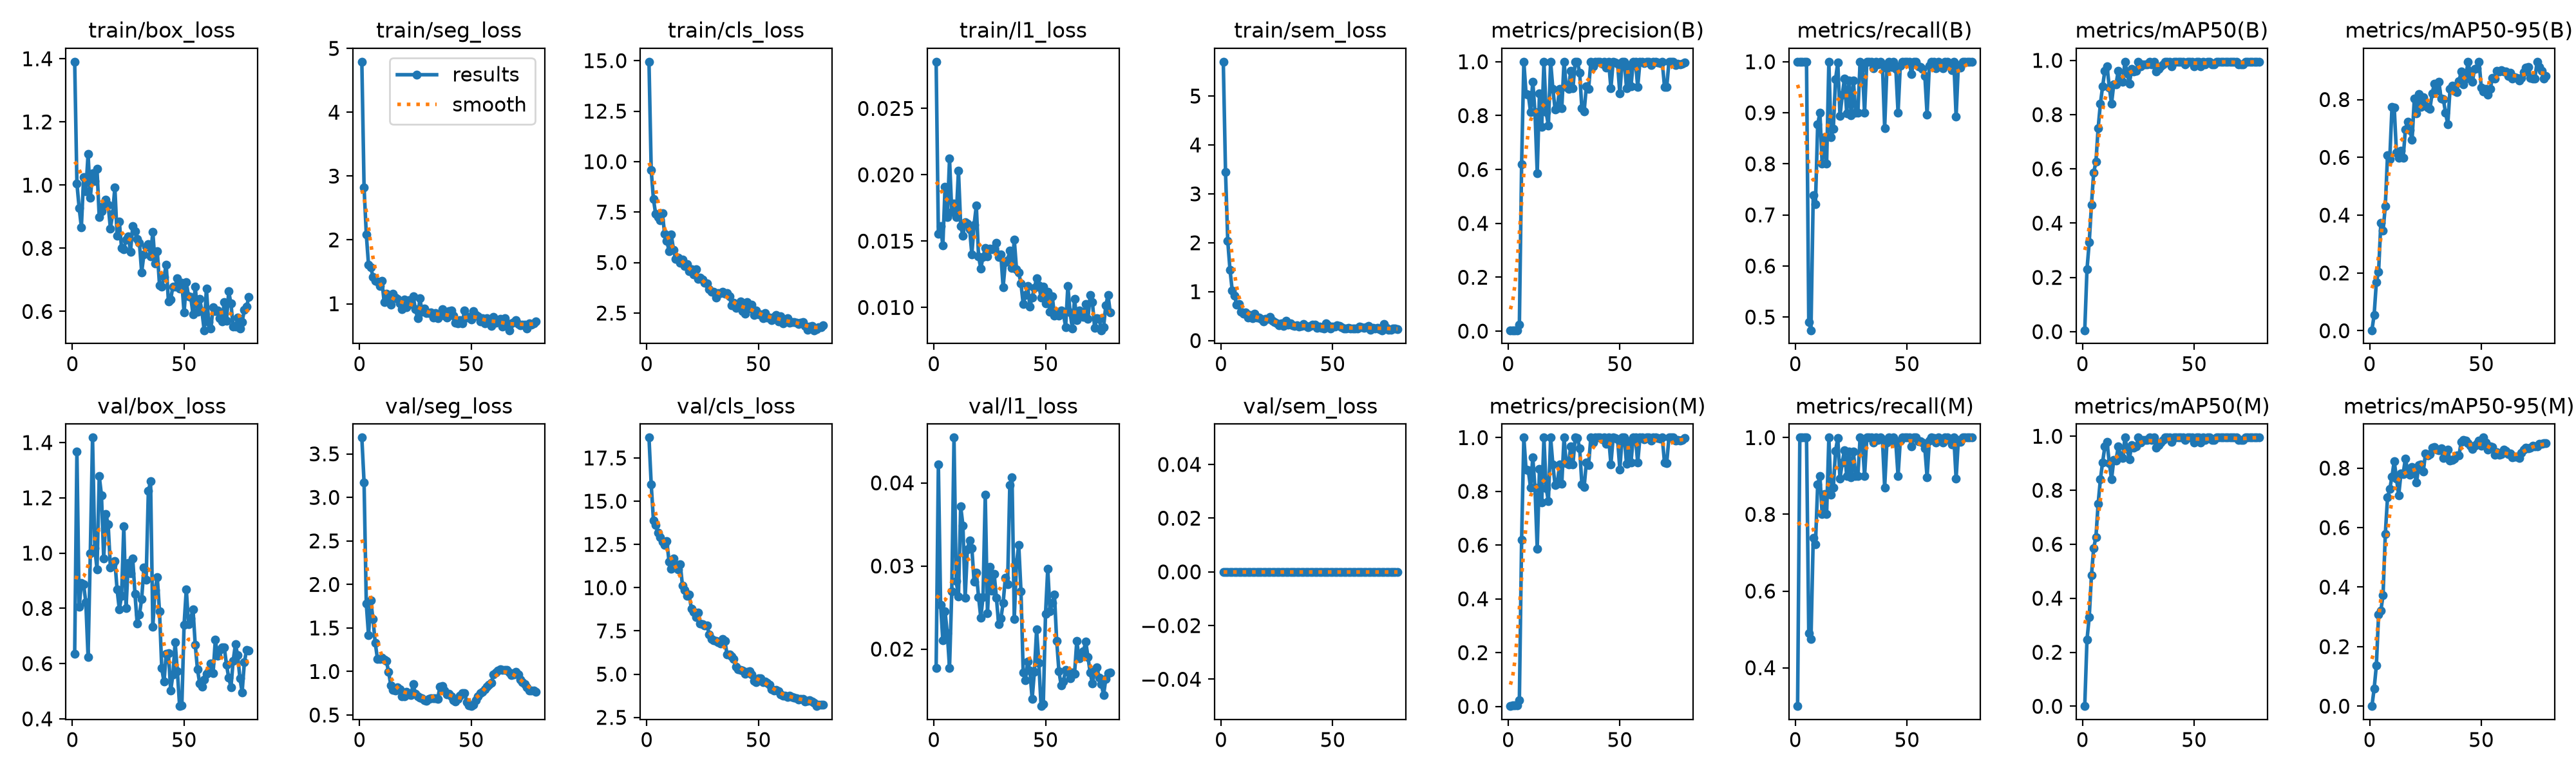
\includegraphics[width=0.95\linewidth]{figures/training_results.png}
\caption{Training curves for the main frozen-backbone run: training losses decrease smoothly and validation mAP converges to high values.}\label{fig:results}
\end{figure}

\begin{figure}[htbp]
\centering
\begin{subfigure}[b]{0.48\linewidth}
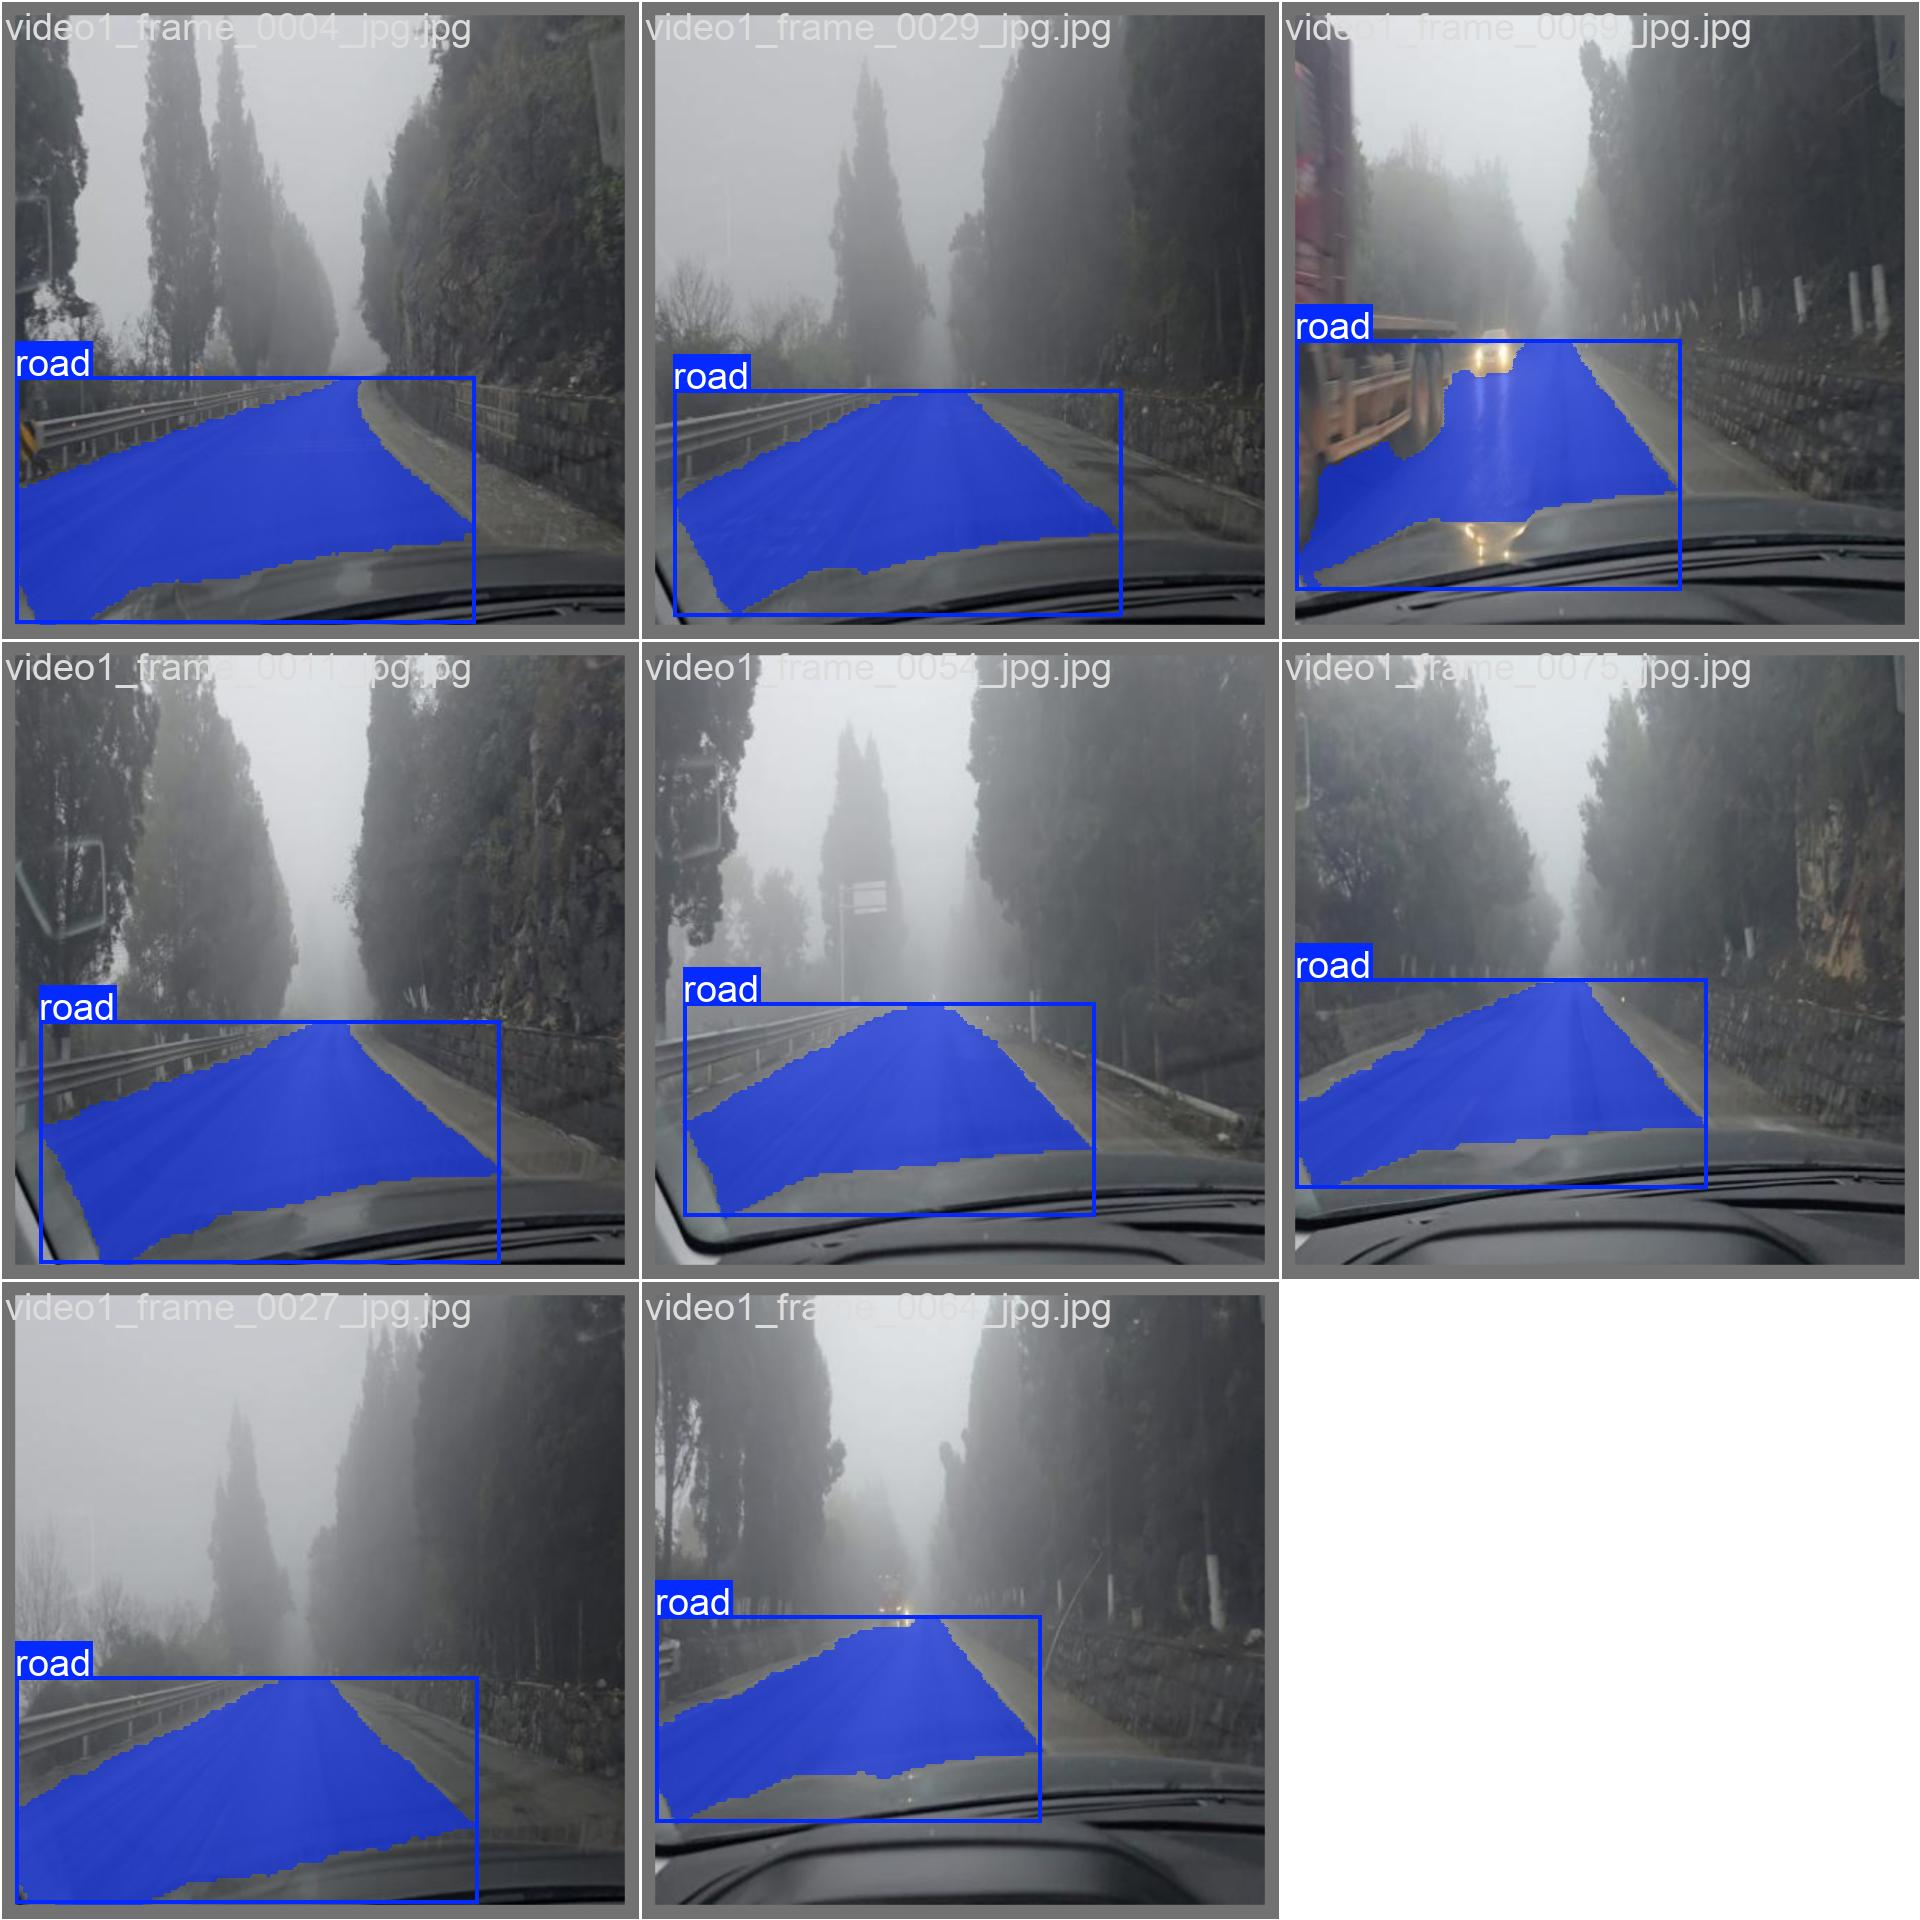
\includegraphics[width=\linewidth]{figures/val_batch0_labels.jpg}
\caption{Ground-truth labels.}
\end{subfigure}
\hfill
\begin{subfigure}[b]{0.48\linewidth}
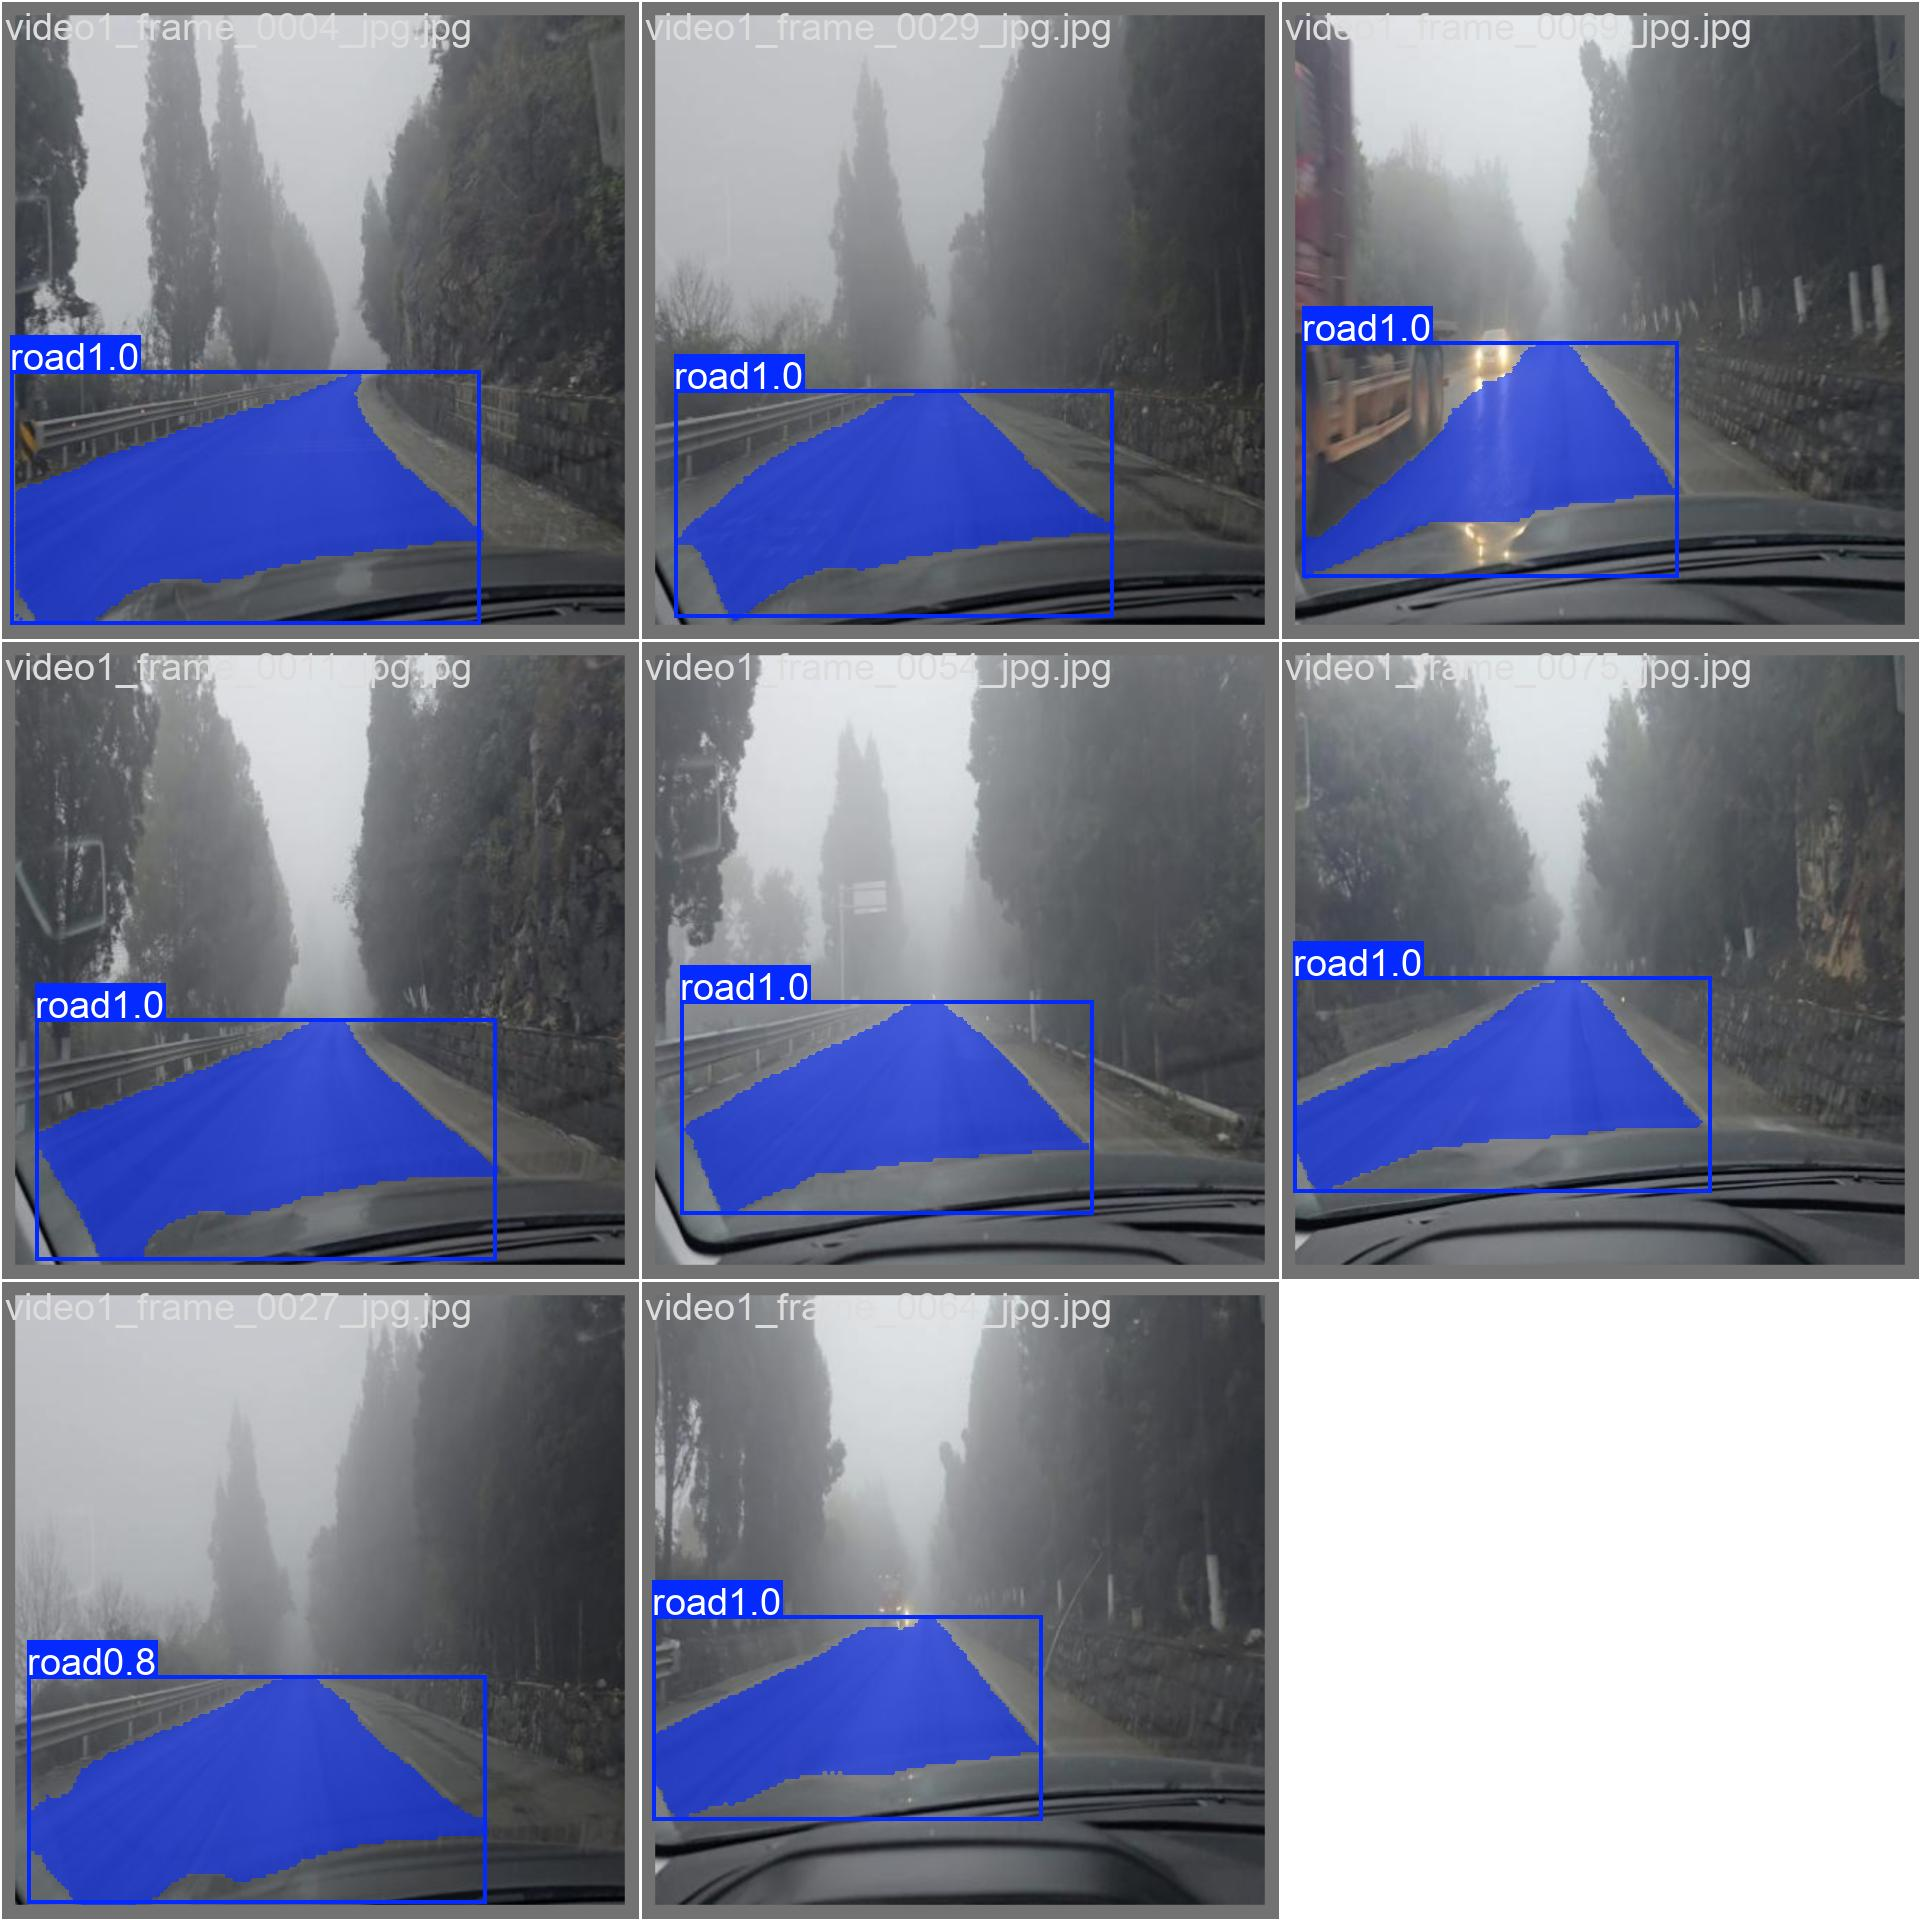
\includegraphics[width=\linewidth]{figures/val_batch0_pred.jpg}
\caption{Model predictions.}
\end{subfigure}
\caption{Qualitative validation results for a batch of road images.}\label{fig:qualitative}
\end{figure}

\subsection{Ablation study: frozen versus unfrozen backbone}

To investigate the effect of transfer learning, we compare models trained with the first 10 layers frozen against models where all layers are unfrozen (full fine-tuning). All other hyperparameters are identical: 120-epoch budget, image size 960, batch size 4, AdamW optimizer, seed 42, and deterministic mode. Each configuration is repeated twice. Results are shown in \cref{tab:ablation}.

\begin{table}[htbp]
\centering
\caption{Backbone-freezing ablation. Each value is the COCO-style validation metric of the best checkpoint.}\label{tab:ablation}
\begin{tabular}{lcccccc}
\toprule
\textbf{Run} & \textbf{Freeze} & \textbf{Box} & \textbf{Box} & \textbf{Mask} & \textbf{Mask} \\
& \textbf{layers} & \textbf{mAP@0.5} & \textbf{mAP@0.5:0.95} & \textbf{mAP@0.5} & \textbf{mAP@0.5:0.95} \\
\midrule
20260731\_115121 & 10  & \textbf{0.995} & \textbf{0.950} & \textbf{0.995} & \textbf{0.879} \\
20260731\_113822 & 10  & 0.909 & 0.770 & 0.905 & 0.764 \\
\midrule
Average frozen    & 10  & 0.952 & 0.860 & 0.950 & 0.822 \\
\midrule
20260731\_101913 & --- & 0.911 & 0.798 & 0.905 & 0.726 \\
20260731\_092953 & --- & 0.909 & 0.755 & 0.905 & 0.766 \\
\midrule
Average unfrozen  & --- & 0.910 & 0.777 & 0.905 & 0.746 \\
\bottomrule
\end{tabular}
\end{table}

On average, freezing the backbone improves box mAP@0.5:0.95 from 0.777 to 0.860 and mask mAP@0.5:0.95 from 0.746 to 0.822. The improvement is most pronounced for the strict mAP metric, which is sensitive to precise boundary alignment. We attribute this to the small target dataset: fine-tuning the entire network has more capacity to overfit training idiosyncrasies, whereas a frozen backbone preserves low-level features learned from COCO and restricts the optimizer to adapt only the task-specific neck and head. The first frozen run (20260731\_115121) is an exceptionally strong outlier; we report it as the best result while emphasizing the averaged trend across repeated runs.

\subsection{Inference resolution and speed}

Training at high resolution improves boundary learning, but inference resolution directly affects latency. We validate the best model at 640$\times$640 and measure the per-component latency reported by Ultralytics. The speed breakdown is shown in \cref{tab:speed}. Total latency is approximately 26.7\,ms per image at batch size 8, which corresponds to roughly 37 frames per second excluding data-loading overhead. This confirms that the nano-scale model is suitable for real-time edge deployment.

\begin{table}[htbp]
\centering
\caption{Per-image latency breakdown on the validation set at 640$\times$640 (batch size 8).}\label{tab:speed}
\begin{tabular}{lc}
\toprule
\textbf{Stage} & \textbf{Time (ms)} \\
\midrule
Pre-processing  & 3.47 \\
Inference       & 21.38 \\
Post-processing & 1.87 \\
\midrule
Total           & 26.72 \\
\bottomrule
\end{tabular}
\end{table}

\subsection{Test-set inference and ONNX export}

The best checkpoint is applied to the held-out test split of 10 images using \tool{src/predict.py}. All 10 images are processed successfully, and annotated outputs with overlaid road masks are saved under \tool{outputs/predict/}. We also export the trained model to ONNX with \tool{src/export.py}, enabling deployment in inference engines that support the ONNX runtime. The export script supports half-precision, dynamic batch axes, and ONNX simplification.

\section{Conclusion}\label{sec:conclusion}

We have presented a reproducible, lightweight pipeline for single-class road instance segmentation. By combining a YOLO-family nano segmentation model, COCO-seg transfer learning with a frozen backbone, high-resolution training, and a rigorous dataset checker, we achieve box and mask mAP@0.5 of 0.995 on our custom road validation set. Ablation experiments confirm that backbone freezing improves strict mAP on small datasets by reducing overfitting. The complete system, from environment setup to ONNX export, is scripted and timestamped, making experiments easy to reproduce and extend.

Several directions remain for future work. First, the dataset currently contains only 100 images; collecting more diverse scenes (night, rain, highway, rural roads) would improve robustness. Second, extending the pipeline to multiple classes---e.g., road, sidewalk, curb, and lane marking---would move closer to production perception stacks. Third, exporting to TensorRT or ONNX Runtime and profiling on an automotive-grade edge device would provide a more accurate assessment of real-world latency and memory consumption. Finally, integrating the segmentation output with a lane-detection or free-space-estimation module would demonstrate end-to-end utility in an autonomous driving pipeline.

\bibliographystyle{plain}
\bibliography{references}

\end{document}
